% Options for packages loaded elsewhere
\PassOptionsToPackage{unicode}{hyperref}
\PassOptionsToPackage{hyphens}{url}
\PassOptionsToPackage{dvipsnames,svgnames,x11names}{xcolor}
%
\documentclass[
  letterpaper,
  DIV=11,
  numbers=noendperiod]{scrreprt}

\usepackage{amsmath,amssymb}
\usepackage{iftex}
\ifPDFTeX
  \usepackage[T1]{fontenc}
  \usepackage[utf8]{inputenc}
  \usepackage{textcomp} % provide euro and other symbols
\else % if luatex or xetex
  \usepackage{unicode-math}
  \defaultfontfeatures{Scale=MatchLowercase}
  \defaultfontfeatures[\rmfamily]{Ligatures=TeX,Scale=1}
\fi
\usepackage{lmodern}
\ifPDFTeX\else  
    % xetex/luatex font selection
\fi
% Use upquote if available, for straight quotes in verbatim environments
\IfFileExists{upquote.sty}{\usepackage{upquote}}{}
\IfFileExists{microtype.sty}{% use microtype if available
  \usepackage[]{microtype}
  \UseMicrotypeSet[protrusion]{basicmath} % disable protrusion for tt fonts
}{}
\makeatletter
\@ifundefined{KOMAClassName}{% if non-KOMA class
  \IfFileExists{parskip.sty}{%
    \usepackage{parskip}
  }{% else
    \setlength{\parindent}{0pt}
    \setlength{\parskip}{6pt plus 2pt minus 1pt}}
}{% if KOMA class
  \KOMAoptions{parskip=half}}
\makeatother
\usepackage{xcolor}
\setlength{\emergencystretch}{3em} % prevent overfull lines
\setcounter{secnumdepth}{5}
% Make \paragraph and \subparagraph free-standing
\ifx\paragraph\undefined\else
  \let\oldparagraph\paragraph
  \renewcommand{\paragraph}[1]{\oldparagraph{#1}\mbox{}}
\fi
\ifx\subparagraph\undefined\else
  \let\oldsubparagraph\subparagraph
  \renewcommand{\subparagraph}[1]{\oldsubparagraph{#1}\mbox{}}
\fi

\usepackage{color}
\usepackage{fancyvrb}
\newcommand{\VerbBar}{|}
\newcommand{\VERB}{\Verb[commandchars=\\\{\}]}
\DefineVerbatimEnvironment{Highlighting}{Verbatim}{commandchars=\\\{\}}
% Add ',fontsize=\small' for more characters per line
\usepackage{framed}
\definecolor{shadecolor}{RGB}{241,243,245}
\newenvironment{Shaded}{\begin{snugshade}}{\end{snugshade}}
\newcommand{\AlertTok}[1]{\textcolor[rgb]{0.68,0.00,0.00}{#1}}
\newcommand{\AnnotationTok}[1]{\textcolor[rgb]{0.37,0.37,0.37}{#1}}
\newcommand{\AttributeTok}[1]{\textcolor[rgb]{0.40,0.45,0.13}{#1}}
\newcommand{\BaseNTok}[1]{\textcolor[rgb]{0.68,0.00,0.00}{#1}}
\newcommand{\BuiltInTok}[1]{\textcolor[rgb]{0.00,0.23,0.31}{#1}}
\newcommand{\CharTok}[1]{\textcolor[rgb]{0.13,0.47,0.30}{#1}}
\newcommand{\CommentTok}[1]{\textcolor[rgb]{0.37,0.37,0.37}{#1}}
\newcommand{\CommentVarTok}[1]{\textcolor[rgb]{0.37,0.37,0.37}{\textit{#1}}}
\newcommand{\ConstantTok}[1]{\textcolor[rgb]{0.56,0.35,0.01}{#1}}
\newcommand{\ControlFlowTok}[1]{\textcolor[rgb]{0.00,0.23,0.31}{#1}}
\newcommand{\DataTypeTok}[1]{\textcolor[rgb]{0.68,0.00,0.00}{#1}}
\newcommand{\DecValTok}[1]{\textcolor[rgb]{0.68,0.00,0.00}{#1}}
\newcommand{\DocumentationTok}[1]{\textcolor[rgb]{0.37,0.37,0.37}{\textit{#1}}}
\newcommand{\ErrorTok}[1]{\textcolor[rgb]{0.68,0.00,0.00}{#1}}
\newcommand{\ExtensionTok}[1]{\textcolor[rgb]{0.00,0.23,0.31}{#1}}
\newcommand{\FloatTok}[1]{\textcolor[rgb]{0.68,0.00,0.00}{#1}}
\newcommand{\FunctionTok}[1]{\textcolor[rgb]{0.28,0.35,0.67}{#1}}
\newcommand{\ImportTok}[1]{\textcolor[rgb]{0.00,0.46,0.62}{#1}}
\newcommand{\InformationTok}[1]{\textcolor[rgb]{0.37,0.37,0.37}{#1}}
\newcommand{\KeywordTok}[1]{\textcolor[rgb]{0.00,0.23,0.31}{#1}}
\newcommand{\NormalTok}[1]{\textcolor[rgb]{0.00,0.23,0.31}{#1}}
\newcommand{\OperatorTok}[1]{\textcolor[rgb]{0.37,0.37,0.37}{#1}}
\newcommand{\OtherTok}[1]{\textcolor[rgb]{0.00,0.23,0.31}{#1}}
\newcommand{\PreprocessorTok}[1]{\textcolor[rgb]{0.68,0.00,0.00}{#1}}
\newcommand{\RegionMarkerTok}[1]{\textcolor[rgb]{0.00,0.23,0.31}{#1}}
\newcommand{\SpecialCharTok}[1]{\textcolor[rgb]{0.37,0.37,0.37}{#1}}
\newcommand{\SpecialStringTok}[1]{\textcolor[rgb]{0.13,0.47,0.30}{#1}}
\newcommand{\StringTok}[1]{\textcolor[rgb]{0.13,0.47,0.30}{#1}}
\newcommand{\VariableTok}[1]{\textcolor[rgb]{0.07,0.07,0.07}{#1}}
\newcommand{\VerbatimStringTok}[1]{\textcolor[rgb]{0.13,0.47,0.30}{#1}}
\newcommand{\WarningTok}[1]{\textcolor[rgb]{0.37,0.37,0.37}{\textit{#1}}}

\providecommand{\tightlist}{%
  \setlength{\itemsep}{0pt}\setlength{\parskip}{0pt}}\usepackage{longtable,booktabs,array}
\usepackage{calc} % for calculating minipage widths
% Correct order of tables after \paragraph or \subparagraph
\usepackage{etoolbox}
\makeatletter
\patchcmd\longtable{\par}{\if@noskipsec\mbox{}\fi\par}{}{}
\makeatother
% Allow footnotes in longtable head/foot
\IfFileExists{footnotehyper.sty}{\usepackage{footnotehyper}}{\usepackage{footnote}}
\makesavenoteenv{longtable}
\usepackage{graphicx}
\makeatletter
\def\maxwidth{\ifdim\Gin@nat@width>\linewidth\linewidth\else\Gin@nat@width\fi}
\def\maxheight{\ifdim\Gin@nat@height>\textheight\textheight\else\Gin@nat@height\fi}
\makeatother
% Scale images if necessary, so that they will not overflow the page
% margins by default, and it is still possible to overwrite the defaults
% using explicit options in \includegraphics[width, height, ...]{}
\setkeys{Gin}{width=\maxwidth,height=\maxheight,keepaspectratio}
% Set default figure placement to htbp
\makeatletter
\def\fps@figure{htbp}
\makeatother

\KOMAoption{captions}{tableheading}
\makeatletter
\@ifpackageloaded{bookmark}{}{\usepackage{bookmark}}
\makeatother
\makeatletter
\@ifpackageloaded{caption}{}{\usepackage{caption}}
\AtBeginDocument{%
\ifdefined\contentsname
  \renewcommand*\contentsname{Table of contents}
\else
  \newcommand\contentsname{Table of contents}
\fi
\ifdefined\listfigurename
  \renewcommand*\listfigurename{List of Figures}
\else
  \newcommand\listfigurename{List of Figures}
\fi
\ifdefined\listtablename
  \renewcommand*\listtablename{List of Tables}
\else
  \newcommand\listtablename{List of Tables}
\fi
\ifdefined\figurename
  \renewcommand*\figurename{Figure}
\else
  \newcommand\figurename{Figure}
\fi
\ifdefined\tablename
  \renewcommand*\tablename{Table}
\else
  \newcommand\tablename{Table}
\fi
}
\@ifpackageloaded{float}{}{\usepackage{float}}
\floatstyle{ruled}
\@ifundefined{c@chapter}{\newfloat{codelisting}{h}{lop}}{\newfloat{codelisting}{h}{lop}[chapter]}
\floatname{codelisting}{Listing}
\newcommand*\listoflistings{\listof{codelisting}{List of Listings}}
\makeatother
\makeatletter
\makeatother
\makeatletter
\@ifpackageloaded{caption}{}{\usepackage{caption}}
\@ifpackageloaded{subcaption}{}{\usepackage{subcaption}}
\makeatother
\ifLuaTeX
  \usepackage{selnolig}  % disable illegal ligatures
\fi
\usepackage{bookmark}

\IfFileExists{xurl.sty}{\usepackage{xurl}}{} % add URL line breaks if available
\urlstyle{same} % disable monospaced font for URLs
\hypersetup{
  pdftitle={Atelier sur LLM - Revolution IA 2024},
  pdfauthor={Simon-Pierre Boucher},
  colorlinks=true,
  linkcolor={blue},
  filecolor={Maroon},
  citecolor={Blue},
  urlcolor={Blue},
  pdfcreator={LaTeX via pandoc}}

\title{Atelier sur LLM - Revolution IA 2024}
\author{Simon-Pierre Boucher}
\date{Invalid Date}

\begin{document}
\maketitle

\renewcommand*\contentsname{Table of contents}
{
\hypersetup{linkcolor=}
\setcounter{tocdepth}{2}
\tableofcontents
}
\bookmarksetup{startatroot}

\chapter*{Preface}\label{preface}
\addcontentsline{toc}{chapter}{Preface}

\markboth{Preface}{Preface}

Bienvenue à notre atelier dédié aux Large Language Models (LLM), une
exploration fascinante à l'intersection de l'intelligence artificielle,
du traitement automatique du langage naturel et de l'apprentissage
automatique. Dans un monde numérique en constante évolution, les LLM
s'avèrent être des outils puissants, capables de comprendre,
d'interpréter et de générer du langage humain de manière cohérente et
contextuellement pertinente.

\section*{Qu'est-ce qu'un Large Language Model
?}\label{quest-ce-quun-large-language-model}
\addcontentsline{toc}{section}{Qu'est-ce qu'un Large Language Model ?}

\markright{Qu'est-ce qu'un Large Language Model ?}

Un Large Language Model est un type de modèle d'intelligence
artificielle qui a été entraîné sur d'énormes ensembles de données
textuelles. Grâce à cet entraînement, ces modèles sont capables de
réaliser une multitude de tâches liées au langage, telles que la
traduction automatique, la génération de texte, la compréhension de
questions et de réponses, et bien plus encore. Les LLM, tels que GPT
(Generative Pre-trained Transformer) d'OpenAI, ont révolutionné la
manière dont nous interagissons avec la technologie, ouvrant la voie à
de nouvelles applications et services innovants.

\section*{Pourquoi cet atelier est-il pertinent
?}\label{pourquoi-cet-atelier-est-il-pertinent}
\addcontentsline{toc}{section}{Pourquoi cet atelier est-il pertinent ?}

\markright{Pourquoi cet atelier est-il pertinent ?}

L'essor des LLM transforme divers secteurs, allant de l'éducation à la
santé, en passant par le service client et le divertissement. Comprendre
le fonctionnement de ces modèles, leurs capacités, leurs limites, et
surtout, leur potentiel pour résoudre des problèmes complexes, est
devenu indispensable pour les professionnels, les chercheurs et les
passionnés de technologie.

Cet atelier a été conçu pour vous fournir une compréhension approfondie
des LLM, à travers des présentations théoriques, des études de cas, et
des sessions pratiques. Vous découvrirez comment ces modèles sont
construits, comment ils apprennent à partir des données et comment ils
peuvent être appliqués pour créer des solutions innovantes.

\subsection*{Objectifs de l'atelier}\label{objectifs-de-latelier}
\addcontentsline{toc}{subsection}{Objectifs de l'atelier}

\begin{itemize}
\tightlist
\item
  \textbf{Comprendre les Fondements des LLM} : Acquérir une connaissance
  solide des principes sous-jacents des LLM, y compris leur architecture
  et leur processus d'entraînement.
\item
  \textbf{Explorer les Applications des LLM} : Découvrir comment les LLM
  sont utilisés dans divers domaines pour améliorer l'efficacité, la
  créativité et la prise de décision.
\item
  \textbf{Développer des Compétences Pratiques} : Appliquer vos
  connaissances à travers des ateliers pratiques, vous permettant de
  mettre en œuvre des LLM pour vos propres projets ou recherches.
\end{itemize}

Nous sommes à l'aube d'une nouvelle ère de l'intelligence artificielle,
où les LLM jouent un rôle central. Rejoignez-nous pour cet atelier afin
d'explorer le potentiel de ces technologies transformatrices et de vous
préparer à contribuer à l'avenir de l'IA.

Nous avons hâte de vous accueillir et de partager avec vous cette
aventure passionnante !

\bookmarksetup{startatroot}

\chapter{Les Transformers : Révolution dans le Traitement Automatique du
Langage
Naturel}\label{les-transformers-ruxe9volution-dans-le-traitement-automatique-du-langage-naturel}

Les Transformers ont révolutionné le champ de l'intelligence
artificielle (IA) et du traitement automatique du langage naturel (TALN)
depuis leur introduction en 2017 par Vaswani et al.~dans le papier
intitulé ``Attention Is All You Need''. Cette architecture novatrice a
permis de faire des avancées significatives dans la compréhension et la
génération du langage naturel, dépassant les performances des modèles
basés sur les réseaux de neurones récurrents (RNN) et les réseaux de
neurones convolutifs (CNN) pour de nombreuses tâches.

\section{Qu'est-ce qu'un Transformer ?}\label{quest-ce-quun-transformer}

Un Transformer est un modèle basé sur le mécanisme d'attention, conçu
pour traiter séquentiellement des données avec une efficacité et une
flexibilité remarquables. Contrairement aux approches précédentes, qui
traitent les séquences mot par mot de manière séquentielle, le
Transformer permet un parallélisme complet de traitement, ce qui réduit
considérablement les temps de formation.

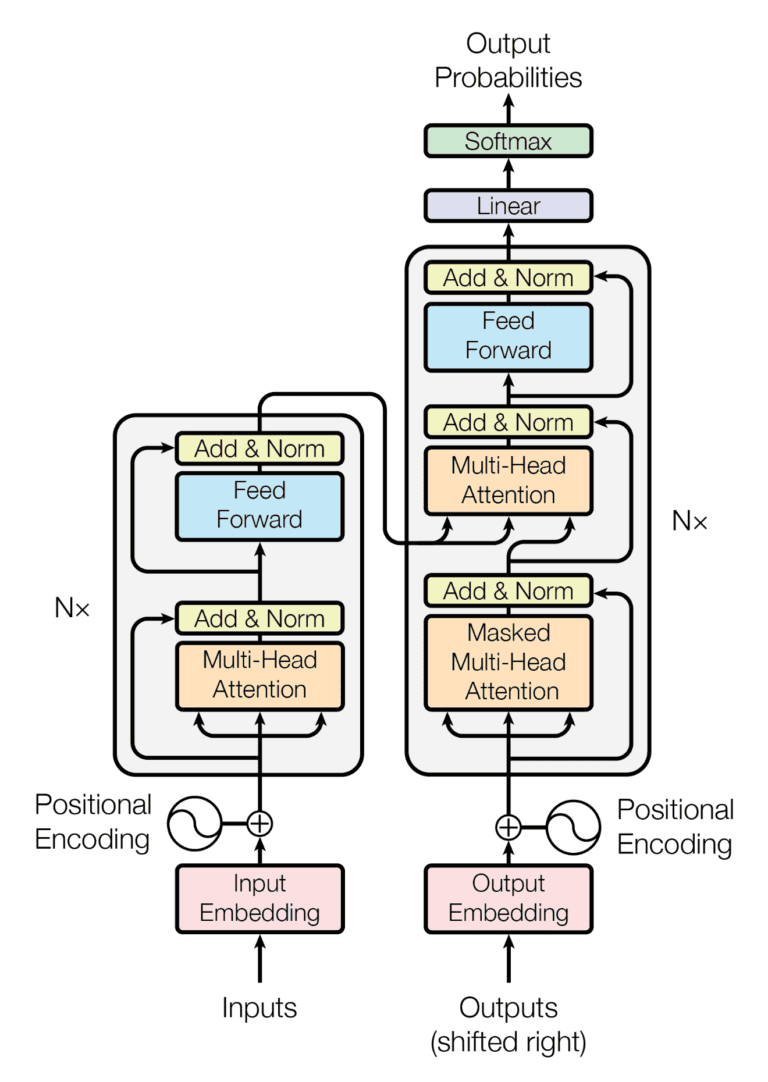
\includegraphics{images/attention_research_1-768x1082.png}

\subsection{Le Mécanisme d'Attention}\label{le-muxe9canisme-dattention}

Le cœur du Transformer est le mécanisme d'attention, spécifiquement
l'attention multi-têtes. Ce mécanisme permet au modèle de se concentrer
sur différentes parties d'une séquence d'entrée lors de la prédiction
d'une partie d'une séquence de sortie, améliorant ainsi sa capacité à
comprendre les relations complexes et lointaines dans les données
textuelles.

\subsection{Architecture du
Transformer}\label{architecture-du-transformer}

L'architecture du Transformer est constituée de deux parties principales
: l'encodeur et le décodeur.

\begin{itemize}
\item
  \textbf{L'Encodeur} : Il traite la séquence d'entrée et la transforme
  en une série de représentations qui contiennent à la fois les
  informations du mot spécifique et le contexte dans lequel il apparaît.
  Chaque couche de l'encodeur contient deux sous-couches : une
  sous-couche d'attention multi-têtes et une sous-couche de réseau de
  neurones entièrement connecté.

  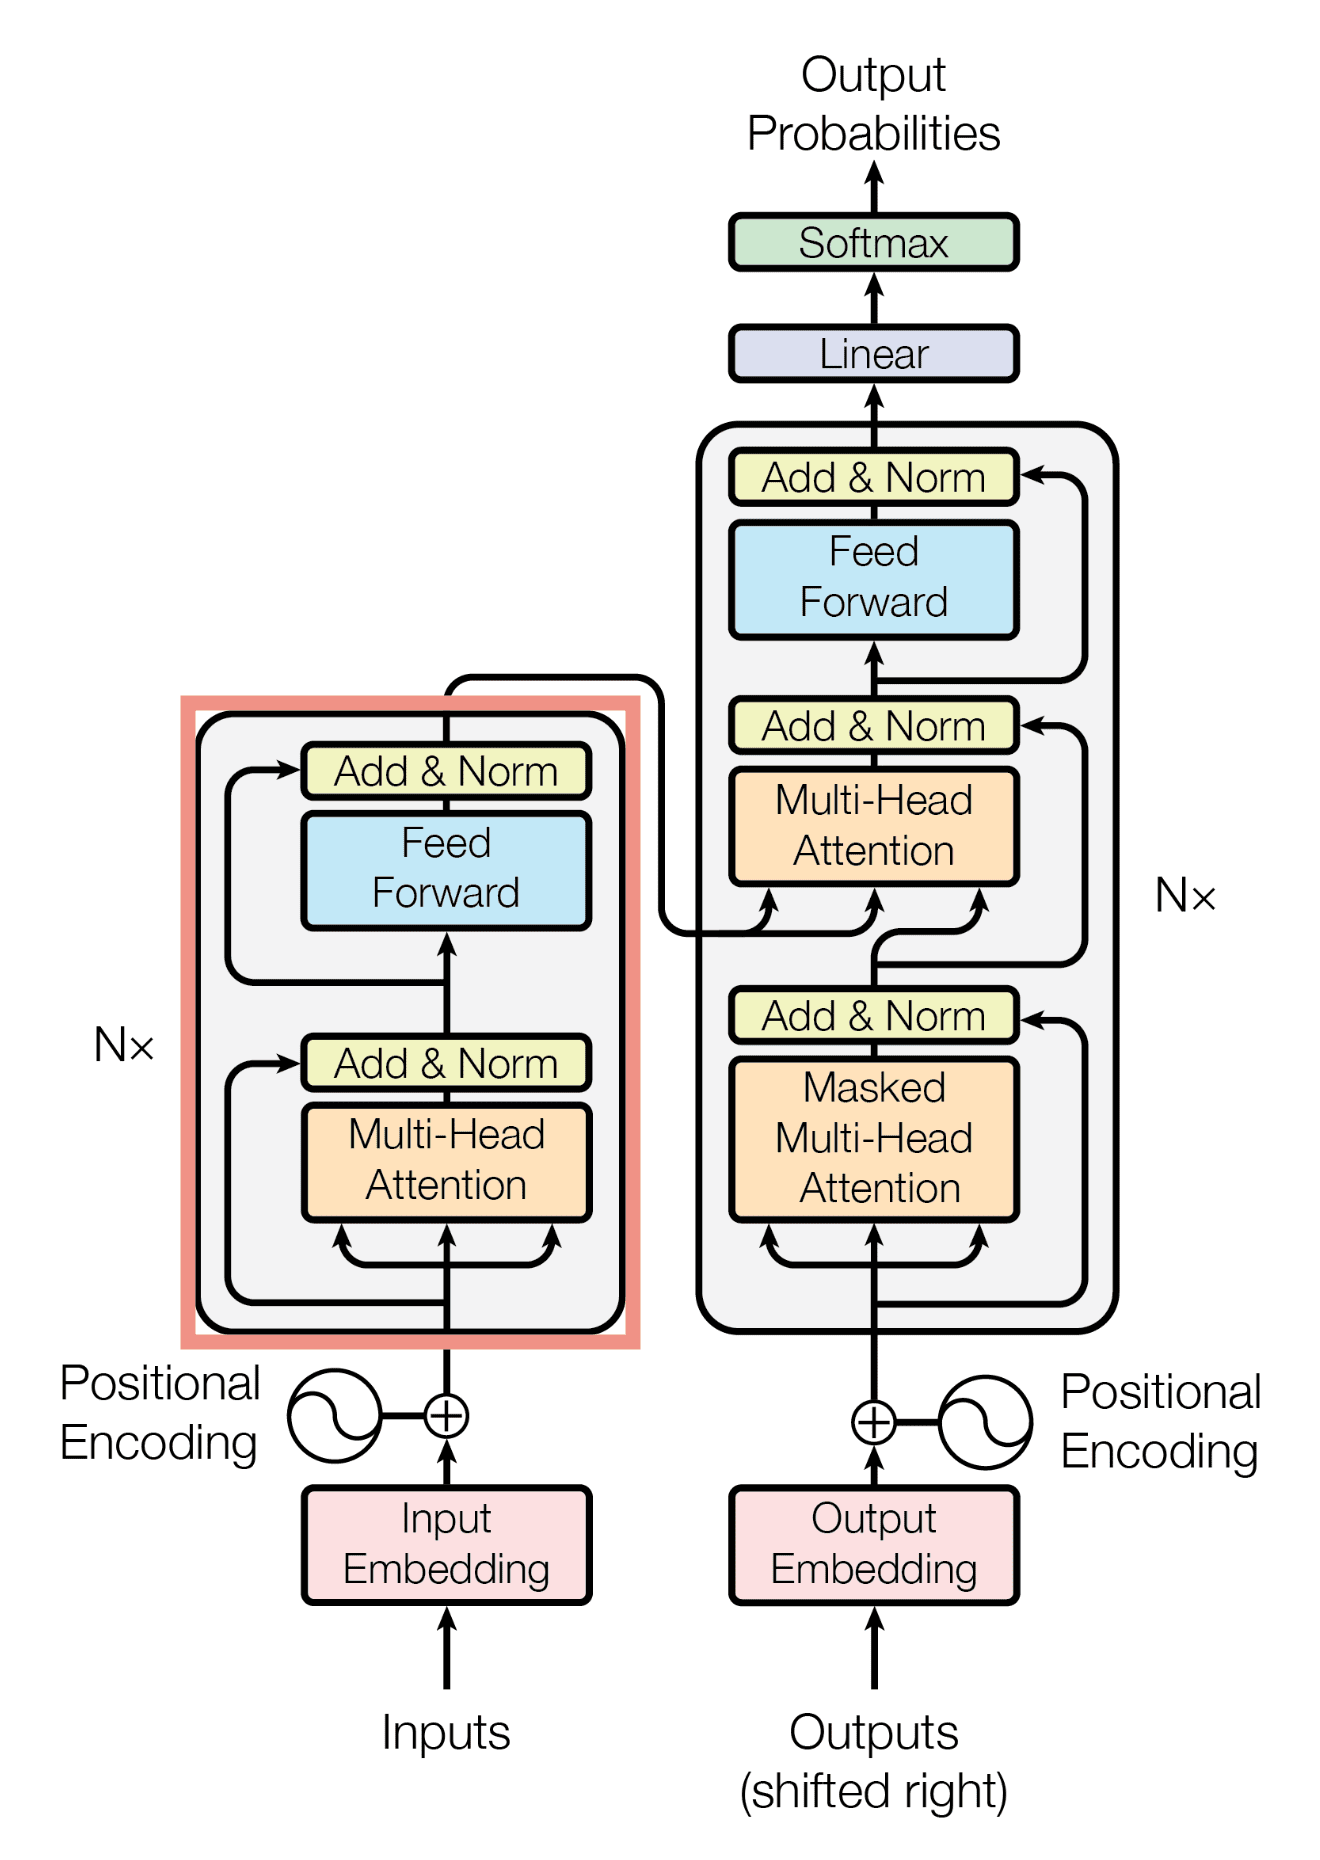
\includegraphics{images/transformer_1.png}
\item
  \textbf{Le Décodeur} : Il génère la séquence de sortie, mot par mot,
  en se basant sur les représentations fournies par l'encodeur et ce qui
  a déjà été généré. Le décodeur ajoute une troisième sous-couche à
  celles trouvées dans l'encodeur, qui permet d'appliquer l'attention
  sur la sortie de l'encodeur.

  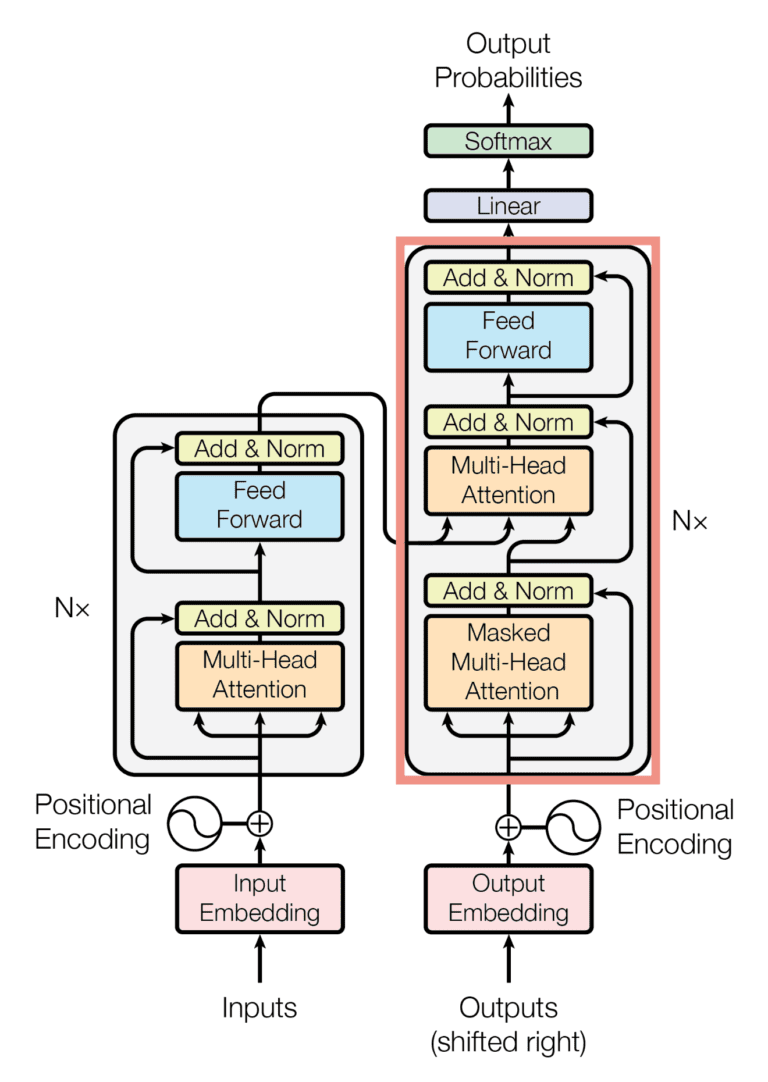
\includegraphics{images/transformer_2-768x1082.png}
\end{itemize}

\section{Avantages des Transformers}\label{avantages-des-transformers}

Les Transformers offrent plusieurs avantages significatifs par rapport
aux architectures précédentes :

\begin{itemize}
\tightlist
\item
  \textbf{Traitement Parallèle} : La capacité à traiter l'ensemble de la
  séquence d'entrée en parallèle conduit à une formation plus rapide des
  modèles.
\item
  \textbf{Gestion des Dépendances à Long Terme} : L'attention
  multi-têtes permet au modèle de se concentrer sur l'ensemble de la
  séquence d'entrée pour chaque mot de la séquence de sortie, gérant
  efficacement les dépendances à long terme.
\item
  \textbf{Flexibilité et Adaptabilité} : Les Transformers ont été
  adaptés avec succès à une grande variété de tâches TALN, y compris la
  traduction automatique, la synthèse de texte et la compréhension de
  texte.
\end{itemize}

\section{Impact des Transformers}\label{impact-des-transformers}

L'introduction des Transformers a marqué un tournant dans le domaine de
l'IA et du TALN. Des modèles comme BERT (Bidirectional Encoder
Representations from Transformers), GPT (Generative Pretrained
Transformer), et d'autres ont établi de nouveaux standards de
performance sur divers benchmarks TALN. Ces modèles ont non seulement
amélioré la qualité de la compréhension et de la génération de texte,
mais ils ont également ouvert la voie à des applications innovantes dans
le traitement du langage naturel, la recherche d'informations, et bien
au-delà.

En somme, les Transformers représentent une avancée majeure dans notre
capacité à modéliser et à comprendre le langage humain, conduisant à des
progrès significatifs dans de nombreuses applications pratiques de l'IA.

\bookmarksetup{startatroot}

\chapter{Acteurs Majeurs dans le Monde de
l'IA}\label{acteurs-majeurs-dans-le-monde-de-lia}

L'univers de l'intelligence artificielle (IA) est peuplé de plusieurs
acteurs majeurs, chacun contribuant de manière significative à
l'avancement et à la démocratisation de la technologie. Voici
quelques-uns des plus influents :

\section{TensorFlow \& Keras}\label{tensorflow-keras}

\begin{itemize}
\item
  \textbf{TensorFlow} : Développé par l'équipe Google Brain, TensorFlow
  est un framework open-source pour le calcul numérique qui facilite la
  construction, le déploiement et la formation de modèles
  d'apprentissage profond. Il est particulièrement connu pour sa
  flexibilité et sa capacité à opérer à grande échelle, ce qui le rend
  populaire parmi les chercheurs et les développeurs travaillant sur des
  projets complexes d'IA.
\item
  \textbf{Keras} : Intégré dans TensorFlow comme \texttt{tf.keras},
  Keras est une interface de haut niveau pour les réseaux de neurones,
  conçue pour l'expérimentation rapide. Facile à utiliser et intuitif,
  Keras permet de construire et de tester des modèles d'IA avec un
  minimum de code, le rendant accessible aux novices tout en restant
  suffisamment puissant pour les chercheurs expérimentés.
\end{itemize}


\includegraphics{images/tensorflowkeras.jpg}

\section{Hugging Face}\label{hugging-face}

Hugging Face est une entreprise technologique qui a pris une importance
considérable dans le monde de l'IA grâce à sa plateforme collaborative
et sa bibliothèque de modèles de traitement automatique du langage
naturel (TALN), \texttt{transformers}. Offrant un accès facile à plus
d'une centaine de modèles pré-entraînés et supportant une multitude de
langues, Hugging Face démocratise l'accès aux technologies d'IA de
pointe. Elle est devenue incontournable pour les chercheurs, les
développeurs, et les entreprises souhaitant intégrer des capacités
avancées de TALN dans leurs applications.


\includegraphics{images/hf-logo.png}

\section{Mistral}\label{mistral}

Mistral est une initiative moins connue mais tout aussi importante dans
le domaine de l'IA, se concentrant sur le développement et
l'optimisation de modèles d'IA pour des performances et une efficacité
énergétique accrues. Bien que moins médiatisée que les autres entités
mentionnées ici, Mistral joue un rôle crucial dans la recherche de
solutions d'IA plus durables et accessibles, en particulier dans des
contextes où les ressources de calcul sont limitées.

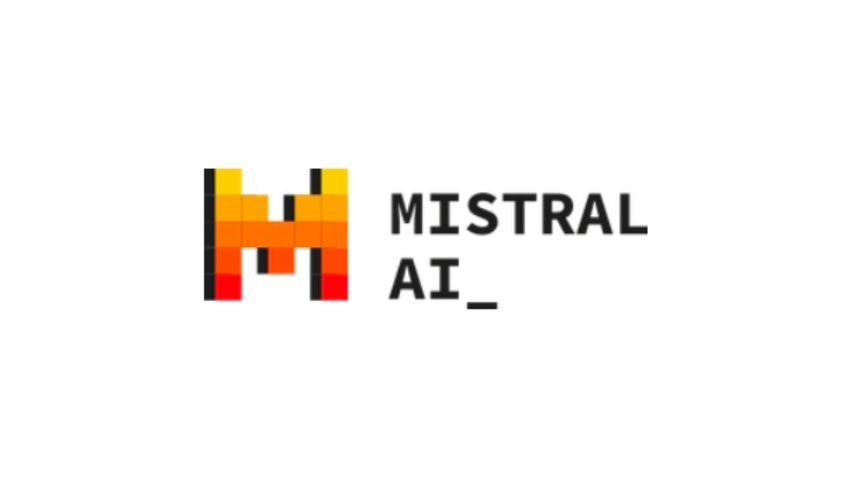
\includegraphics{images/News_Image_-_2023-12-11T192644.220.jpeg}

\section{OpenAI}\label{openai}

OpenAI est une organisation de recherche en IA fondée avec l'objectif de
promouvoir et de développer une intelligence artificielle amicale de
manière à bénéficier à l'humanité dans son ensemble. Connue pour ses
travaux de recherche de pointe et ses publications influentes, OpenAI a
développé des modèles d'IA révolutionnaires comme GPT (Generative
Pretrained Transformer) et DALL·E. Par ses contributions, OpenAI
influence profondément la direction de la recherche en IA et le
développement d'applications innovantes, tout en suscitant un débat
public sur les implications éthiques et sociétales de l'IA avancée.

Chacun de ces acteurs joue un rôle distinct dans l'écosystème de l'IA,
contribuant à son avancement et à sa démocratisation. Que ce soit par le
développement de frameworks et d'outils accessibles, la mise à
disposition de modèles pré-entraînés, la recherche fondamentale, ou la
sensibilisation aux enjeux éthiques, ils façonnent ensemble l'avenir de
l'intelligence artificielle.

\includegraphics{images/6138535.webp}

\bookmarksetup{startatroot}

\chapter{Architecture du modèle}\label{architecture-du-moduxe8le}

La plupart des modèles neuronaux de transduction de séquences
compétitifs possèdent une structure encodeur-décodeur
\href{https://arxiv.org/abs/1409.0473}{(cite)}. Ici, l'encodeur associe
une séquence d'entrée de représentations symboliques \((x_1, ..., x_n)\)
à une séquence de représentations continues
\(\mathbf{z} = (z_1, ..., z_n)\). Étant donné \(\mathbf{z}\), le
décodeur génère ensuite une séquence de sortie \((y_1,...,y_m)\) de
symboles, un élément à la fois. À chaque étape, le modèle est
auto-régressif \href{https://arxiv.org/abs/1308.0850}{(cite)}, utilisant
les symboles précédemment générés comme entrée supplémentaire lors de la
génération du suivant.

\begin{Shaded}
\begin{Highlighting}[]
\KeywordTok{class}\NormalTok{ EncoderDecoder(nn.Module):}
    \CommentTok{"""}
\CommentTok{    A standard Encoder{-}Decoder architecture. Base for this and many}
\CommentTok{    other models.}
\CommentTok{    """}

    \KeywordTok{def} \FunctionTok{\_\_init\_\_}\NormalTok{(}\VariableTok{self}\NormalTok{, encoder, decoder, src\_embed, tgt\_embed, generator):}
        \BuiltInTok{super}\NormalTok{(EncoderDecoder, }\VariableTok{self}\NormalTok{).}\FunctionTok{\_\_init\_\_}\NormalTok{()}
        \VariableTok{self}\NormalTok{.encoder }\OperatorTok{=}\NormalTok{ encoder}
        \VariableTok{self}\NormalTok{.decoder }\OperatorTok{=}\NormalTok{ decoder}
        \VariableTok{self}\NormalTok{.src\_embed }\OperatorTok{=}\NormalTok{ src\_embed}
        \VariableTok{self}\NormalTok{.tgt\_embed }\OperatorTok{=}\NormalTok{ tgt\_embed}
        \VariableTok{self}\NormalTok{.generator }\OperatorTok{=}\NormalTok{ generator}

    \KeywordTok{def}\NormalTok{ forward(}\VariableTok{self}\NormalTok{, src, tgt, src\_mask, tgt\_mask):}
        \CommentTok{"Take in and process masked src and target sequences."}
        \ControlFlowTok{return} \VariableTok{self}\NormalTok{.decode(}\VariableTok{self}\NormalTok{.encode(src, src\_mask), src\_mask, tgt, tgt\_mask)}

    \KeywordTok{def}\NormalTok{ encode(}\VariableTok{self}\NormalTok{, src, src\_mask):}
        \ControlFlowTok{return} \VariableTok{self}\NormalTok{.encoder(}\VariableTok{self}\NormalTok{.src\_embed(src), src\_mask)}

    \KeywordTok{def}\NormalTok{ decode(}\VariableTok{self}\NormalTok{, memory, src\_mask, tgt, tgt\_mask):}
        \ControlFlowTok{return} \VariableTok{self}\NormalTok{.decoder(}\VariableTok{self}\NormalTok{.tgt\_embed(tgt), memory, src\_mask, tgt\_mask)}
        
      
\KeywordTok{class}\NormalTok{ Generator(nn.Module):}
    \CommentTok{"Define standard linear + softmax generation step."}

    \KeywordTok{def} \FunctionTok{\_\_init\_\_}\NormalTok{(}\VariableTok{self}\NormalTok{, d\_model, vocab):}
        \BuiltInTok{super}\NormalTok{(Generator, }\VariableTok{self}\NormalTok{).}\FunctionTok{\_\_init\_\_}\NormalTok{()}
        \VariableTok{self}\NormalTok{.proj }\OperatorTok{=}\NormalTok{ nn.Linear(d\_model, vocab)}

    \KeywordTok{def}\NormalTok{ forward(}\VariableTok{self}\NormalTok{, x):}
        \ControlFlowTok{return}\NormalTok{ log\_softmax(}\VariableTok{self}\NormalTok{.proj(x), dim}\OperatorTok{={-}}\DecValTok{1}\NormalTok{)}
\end{Highlighting}
\end{Shaded}

\section{Encodeur et Décodeur}\label{encodeur-et-duxe9codeur}

\subsection{Encodeur}\label{encodeur}

L'encodeur est composé d'une pile de \(N=6\) couches identiques.

\begin{Shaded}
\begin{Highlighting}[]
\KeywordTok{def}\NormalTok{ clones(module, N):}
    \CommentTok{"Produce N identical layers."}
    \ControlFlowTok{return}\NormalTok{ nn.ModuleList([copy.deepcopy(module) }\ControlFlowTok{for}\NormalTok{ \_ }\KeywordTok{in} \BuiltInTok{range}\NormalTok{(N)])}
    

\KeywordTok{class}\NormalTok{ Encoder(nn.Module):}
    \CommentTok{"Core encoder is a stack of N layers"}

    \KeywordTok{def} \FunctionTok{\_\_init\_\_}\NormalTok{(}\VariableTok{self}\NormalTok{, layer, N):}
        \BuiltInTok{super}\NormalTok{(Encoder, }\VariableTok{self}\NormalTok{).}\FunctionTok{\_\_init\_\_}\NormalTok{()}
        \VariableTok{self}\NormalTok{.layers }\OperatorTok{=}\NormalTok{ clones(layer, N)}
        \VariableTok{self}\NormalTok{.norm }\OperatorTok{=}\NormalTok{ LayerNorm(layer.size)}

    \KeywordTok{def}\NormalTok{ forward(}\VariableTok{self}\NormalTok{, x, mask):}
        \CommentTok{"Pass the input (and mask) through each layer in turn."}
        \ControlFlowTok{for}\NormalTok{ layer }\KeywordTok{in} \VariableTok{self}\NormalTok{.layers:}
\NormalTok{            x }\OperatorTok{=}\NormalTok{ layer(x, mask)}
        \ControlFlowTok{return} \VariableTok{self}\NormalTok{.norm(x)}
        
\KeywordTok{class}\NormalTok{ LayerNorm(nn.Module):}
    \CommentTok{"Construct a layernorm module (See citation for details)."}

    \KeywordTok{def} \FunctionTok{\_\_init\_\_}\NormalTok{(}\VariableTok{self}\NormalTok{, features, eps}\OperatorTok{=}\FloatTok{1e{-}6}\NormalTok{):}
        \BuiltInTok{super}\NormalTok{(LayerNorm, }\VariableTok{self}\NormalTok{).}\FunctionTok{\_\_init\_\_}\NormalTok{()}
        \VariableTok{self}\NormalTok{.a\_2 }\OperatorTok{=}\NormalTok{ nn.Parameter(torch.ones(features))}
        \VariableTok{self}\NormalTok{.b\_2 }\OperatorTok{=}\NormalTok{ nn.Parameter(torch.zeros(features))}
        \VariableTok{self}\NormalTok{.eps }\OperatorTok{=}\NormalTok{ eps}

    \KeywordTok{def}\NormalTok{ forward(}\VariableTok{self}\NormalTok{, x):}
\NormalTok{        mean }\OperatorTok{=}\NormalTok{ x.mean(}\OperatorTok{{-}}\DecValTok{1}\NormalTok{, keepdim}\OperatorTok{=}\VariableTok{True}\NormalTok{)}
\NormalTok{        std }\OperatorTok{=}\NormalTok{ x.std(}\OperatorTok{{-}}\DecValTok{1}\NormalTok{, keepdim}\OperatorTok{=}\VariableTok{True}\NormalTok{)}
        \ControlFlowTok{return} \VariableTok{self}\NormalTok{.a\_2 }\OperatorTok{*}\NormalTok{ (x }\OperatorTok{{-}}\NormalTok{ mean) }\OperatorTok{/}\NormalTok{ (std }\OperatorTok{+} \VariableTok{self}\NormalTok{.eps) }\OperatorTok{+} \VariableTok{self}\NormalTok{.b\_2}
        

\KeywordTok{class}\NormalTok{ SublayerConnection(nn.Module):}
    \CommentTok{"""}
\CommentTok{    A residual connection followed by a layer norm.}
\CommentTok{    Note for code simplicity the norm is first as opposed to last.}
\CommentTok{    """}

    \KeywordTok{def} \FunctionTok{\_\_init\_\_}\NormalTok{(}\VariableTok{self}\NormalTok{, size, dropout):}
        \BuiltInTok{super}\NormalTok{(SublayerConnection, }\VariableTok{self}\NormalTok{).}\FunctionTok{\_\_init\_\_}\NormalTok{()}
        \VariableTok{self}\NormalTok{.norm }\OperatorTok{=}\NormalTok{ LayerNorm(size)}
        \VariableTok{self}\NormalTok{.dropout }\OperatorTok{=}\NormalTok{ nn.Dropout(dropout)}

    \KeywordTok{def}\NormalTok{ forward(}\VariableTok{self}\NormalTok{, x, sublayer):}
        \CommentTok{"Apply residual connection to any sublayer with the same size."}
        \ControlFlowTok{return}\NormalTok{ x }\OperatorTok{+} \VariableTok{self}\NormalTok{.dropout(sublayer(}\VariableTok{self}\NormalTok{.norm(x)))}
        

\KeywordTok{class}\NormalTok{ EncoderLayer(nn.Module):}
    \CommentTok{"Encoder is made up of self{-}attn and feed forward (defined below)"}

    \KeywordTok{def} \FunctionTok{\_\_init\_\_}\NormalTok{(}\VariableTok{self}\NormalTok{, size, self\_attn, feed\_forward, dropout):}
        \BuiltInTok{super}\NormalTok{(EncoderLayer, }\VariableTok{self}\NormalTok{).}\FunctionTok{\_\_init\_\_}\NormalTok{()}
        \VariableTok{self}\NormalTok{.self\_attn }\OperatorTok{=}\NormalTok{ self\_attn}
        \VariableTok{self}\NormalTok{.feed\_forward }\OperatorTok{=}\NormalTok{ feed\_forward}
        \VariableTok{self}\NormalTok{.sublayer }\OperatorTok{=}\NormalTok{ clones(SublayerConnection(size, dropout), }\DecValTok{2}\NormalTok{)}
        \VariableTok{self}\NormalTok{.size }\OperatorTok{=}\NormalTok{ size}

    \KeywordTok{def}\NormalTok{ forward(}\VariableTok{self}\NormalTok{, x, mask):}
        \CommentTok{"Follow Figure 1 (left) for connections."}
\NormalTok{        x }\OperatorTok{=} \VariableTok{self}\NormalTok{.sublayer[}\DecValTok{0}\NormalTok{](x, }\KeywordTok{lambda}\NormalTok{ x: }\VariableTok{self}\NormalTok{.self\_attn(x, x, x, mask))}
        \ControlFlowTok{return} \VariableTok{self}\NormalTok{.sublayer[}\DecValTok{1}\NormalTok{](x, }\VariableTok{self}\NormalTok{.feed\_forward)}
      
      
\end{Highlighting}
\end{Shaded}

\subsection{Decodeur}\label{decodeur}

Le décodeur est également composé d'une pile de \(N=6\) couches
identiques.

\begin{Shaded}
\begin{Highlighting}[]
\KeywordTok{class}\NormalTok{ Decoder(nn.Module):}
    \CommentTok{"Generic N layer decoder with masking."}

    \KeywordTok{def} \FunctionTok{\_\_init\_\_}\NormalTok{(}\VariableTok{self}\NormalTok{, layer, N):}
        \BuiltInTok{super}\NormalTok{(Decoder, }\VariableTok{self}\NormalTok{).}\FunctionTok{\_\_init\_\_}\NormalTok{()}
        \VariableTok{self}\NormalTok{.layers }\OperatorTok{=}\NormalTok{ clones(layer, N)}
        \VariableTok{self}\NormalTok{.norm }\OperatorTok{=}\NormalTok{ LayerNorm(layer.size)}

    \KeywordTok{def}\NormalTok{ forward(}\VariableTok{self}\NormalTok{, x, memory, src\_mask, tgt\_mask):}
        \ControlFlowTok{for}\NormalTok{ layer }\KeywordTok{in} \VariableTok{self}\NormalTok{.layers:}
\NormalTok{            x }\OperatorTok{=}\NormalTok{ layer(x, memory, src\_mask, tgt\_mask)}
        \ControlFlowTok{return} \VariableTok{self}\NormalTok{.norm(x)}
        
  
  \KeywordTok{class}\NormalTok{ DecoderLayer(nn.Module):}
    \CommentTok{"Decoder is made of self{-}attn, src{-}attn, and feed forward (defined below)"}

    \KeywordTok{def} \FunctionTok{\_\_init\_\_}\NormalTok{(}\VariableTok{self}\NormalTok{, size, self\_attn, src\_attn, feed\_forward, dropout):}
        \BuiltInTok{super}\NormalTok{(DecoderLayer, }\VariableTok{self}\NormalTok{).}\FunctionTok{\_\_init\_\_}\NormalTok{()}
        \VariableTok{self}\NormalTok{.size }\OperatorTok{=}\NormalTok{ size}
        \VariableTok{self}\NormalTok{.self\_attn }\OperatorTok{=}\NormalTok{ self\_attn}
        \VariableTok{self}\NormalTok{.src\_attn }\OperatorTok{=}\NormalTok{ src\_attn}
        \VariableTok{self}\NormalTok{.feed\_forward }\OperatorTok{=}\NormalTok{ feed\_forward}
        \VariableTok{self}\NormalTok{.sublayer }\OperatorTok{=}\NormalTok{ clones(SublayerConnection(size, dropout), }\DecValTok{3}\NormalTok{)}

    \KeywordTok{def}\NormalTok{ forward(}\VariableTok{self}\NormalTok{, x, memory, src\_mask, tgt\_mask):}
        \CommentTok{"Follow Figure 1 (right) for connections."}
\NormalTok{        m }\OperatorTok{=}\NormalTok{ memory}
\NormalTok{        x }\OperatorTok{=} \VariableTok{self}\NormalTok{.sublayer[}\DecValTok{0}\NormalTok{](x, }\KeywordTok{lambda}\NormalTok{ x: }\VariableTok{self}\NormalTok{.self\_attn(x, x, x, tgt\_mask))}
\NormalTok{        x }\OperatorTok{=} \VariableTok{self}\NormalTok{.sublayer[}\DecValTok{1}\NormalTok{](x, }\KeywordTok{lambda}\NormalTok{ x: }\VariableTok{self}\NormalTok{.src\_attn(x, m, m, src\_mask))}
        \ControlFlowTok{return} \VariableTok{self}\NormalTok{.sublayer[}\DecValTok{2}\NormalTok{](x, }\VariableTok{self}\NormalTok{.feed\_forward)}
        
  \KeywordTok{def}\NormalTok{ subsequent\_mask(size):}
    \CommentTok{"Mask out subsequent positions."}
\NormalTok{    attn\_shape }\OperatorTok{=}\NormalTok{ (}\DecValTok{1}\NormalTok{, size, size)}
\NormalTok{    subsequent\_mask }\OperatorTok{=}\NormalTok{ torch.triu(torch.ones(attn\_shape), diagonal}\OperatorTok{=}\DecValTok{1}\NormalTok{).}\BuiltInTok{type}\NormalTok{(}
\NormalTok{        torch.uint8}
\NormalTok{    )}
    \ControlFlowTok{return}\NormalTok{ subsequent\_mask }\OperatorTok{==} \DecValTok{0}


\KeywordTok{def}\NormalTok{ example\_mask():}
\NormalTok{    LS\_data }\OperatorTok{=}\NormalTok{ pd.concat(}
\NormalTok{        [}
\NormalTok{            pd.DataFrame(}
\NormalTok{                \{}
                    \StringTok{"Subsequent Mask"}\NormalTok{: subsequent\_mask(}\DecValTok{20}\NormalTok{)[}\DecValTok{0}\NormalTok{][x, y].flatten(),}
                    \StringTok{"Window"}\NormalTok{: y,}
                    \StringTok{"Masking"}\NormalTok{: x,}
\NormalTok{                \}}
\NormalTok{            )}
            \ControlFlowTok{for}\NormalTok{ y }\KeywordTok{in} \BuiltInTok{range}\NormalTok{(}\DecValTok{20}\NormalTok{)}
            \ControlFlowTok{for}\NormalTok{ x }\KeywordTok{in} \BuiltInTok{range}\NormalTok{(}\DecValTok{20}\NormalTok{)}
\NormalTok{        ]}
\NormalTok{    )}

    \ControlFlowTok{return}\NormalTok{ (}
\NormalTok{        alt.Chart(LS\_data)}
\NormalTok{        .mark\_rect()}
\NormalTok{        .properties(height}\OperatorTok{=}\DecValTok{250}\NormalTok{, width}\OperatorTok{=}\DecValTok{250}\NormalTok{)}
\NormalTok{        .encode(}
\NormalTok{            alt.X(}\StringTok{"Window:O"}\NormalTok{),}
\NormalTok{            alt.Y(}\StringTok{"Masking:O"}\NormalTok{),}
\NormalTok{            alt.Color(}\StringTok{"Subsequent Mask:Q"}\NormalTok{, scale}\OperatorTok{=}\NormalTok{alt.Scale(scheme}\OperatorTok{=}\StringTok{"viridis"}\NormalTok{)),}
\NormalTok{        )}
\NormalTok{        .interactive()}
\NormalTok{    )}


\NormalTok{show\_example(example\_mask)}
\end{Highlighting}
\end{Shaded}

\bookmarksetup{startatroot}

\chapter{LoRA Finetuning}\label{lora-finetuning}

\textbf{Low-Rank Adaptation (LoRA)} est une technique innovante conçue
pour le fine-tuning efficace des grands modèles de langage (LLM).
Plongeons dans ce qui fait de LoRA un changement de paradigme dans le
domaine de l'apprentissage automatique et du traitement du langage
naturel :

\section{Qu'est-ce que LoRA ?}\label{quest-ce-que-lora}

\begin{itemize}
\tightlist
\item
  \textbf{Concept :} LoRA introduit une décomposition de bas rang pour
  les matrices de poids au sein des modèles de transformateurs.
\item
  \textbf{Efficacité :} En entraînant seulement un petit nombre de
  paramètres supplémentaires, LoRA réduit considérablement le coût
  computationnel.
\end{itemize}

\section{Avantages de LoRA}\label{avantages-de-lora}

\begin{itemize}
\tightlist
\item
  \textbf{Vitesse :} Le fine-tuning avec LoRA est significativement plus
  rapide en raison du moindre nombre de paramètres mis à jour.
\item
  \textbf{Personnalisation :} Cela permet aux data scientists d'adapter
  de grands modèles à leurs tâches spécifiques sans un réentraînement
  extensif.
\end{itemize}

\section{Quelques Cas d'Usage}\label{quelques-cas-dusage}

\begin{itemize}
\tightlist
\item
  \textbf{IA Personnalisée :} Personnalisez les modèles d'IA pour
  comprendre des jargons ou concepts spécifiques dans des domaines de
  niche.
\item
  \textbf{Performance Optimisée :} Améliorez la performance sur des
  tâches comme l'analyse de sentiments ou le résumé de documents avec un
  fine-tuning spécifique au domaine.
\item
  \textbf{Déploiement Efficace :} Capable de déployer un grand modèle de
  base LLM et plusieurs petits adaptateurs LoRA, au lieu de devoir
  déployer plusieurs grands modèles.
\end{itemize}

Dans les sections suivantes, nous explorerons comment implémenter LoRA
en pratique et verrons ses avantages de première main.

\section{Installation}\label{installation}

\begin{itemize}
\tightlist
\item
  Assurez-vous d'être sur une instance GPU
\item
  Installez les packages requis pour le fine-tuning ; voir le Hub de
  Finetuning LLM
\item
  Installez PEFT depuis la source pour les nouvelles fonctionnalités
\item
  Redémarrez l'instance si nécessaire
\end{itemize}



\end{document}
